\documentclass{article}
\usepackage{amsmath}
\usepackage{tikz}
\usetikzlibrary{automata,positioning}
\title{Theory of Computation \\ Assignment 3}
\author{Michael Carpenter}
\date{\today}
\begin{document}
\maketitle

\begin{itemize}
  \item \textbf{2.1.a -} \\
    $E \Rightarrow T \Rightarrow F \Rightarrow a$
  \item 2.1.b - \\
    $E \Rightarrow E + T \Rightarrow T + T \Rightarrow F + T \Rightarrow F + F \Rightarrow a + F \Rightarrow a + a$
  \item \textbf{2.1.c -} \\
    $E \Rightarrow E + T \Rightarrow E + T + T \Rightarrow T + T + T \Rightarrow F + T + T \Rightarrow$ \\
    $F + F + T \Rightarrow F + F + F \Rightarrow a + F + F \Rightarrow a + a + F \Rightarrow a + a + a$ \\
  \item \textbf{2.1.d -} \\
    $E \Rightarrow T \Rightarrow F \Rightarrow (E) \Rightarrow (T) \Rightarrow (F) \Rightarrow ((E)) \Rightarrow ((T)) \Rightarrow$ \\
    $((F)) \Rightarrow ((a))$
  \item \textbf{2.6.b -} \\
    $S \to AS \mid BS \mid A \mid B \mid C$ \\
    $A \to aAb \mid bAa \mid aA \mid Aa \mid a$ \\
    $B \to aBb \mid bBa \mid bB \mid Bb \mid b$ \\
    $C \to a \mid b$ \\
  \item \textbf{2.6.d -} \\
    $S \to LPR \mid \varepsilon$ \\
    $P \to aPa \mid bPb \mid \varepsilon$ \\
    $L \to P\#L \mid \varepsilon$ \\ 
    $R \to R\#P \mid \varepsilon$ \\
  \item \textbf{2.11 -}
    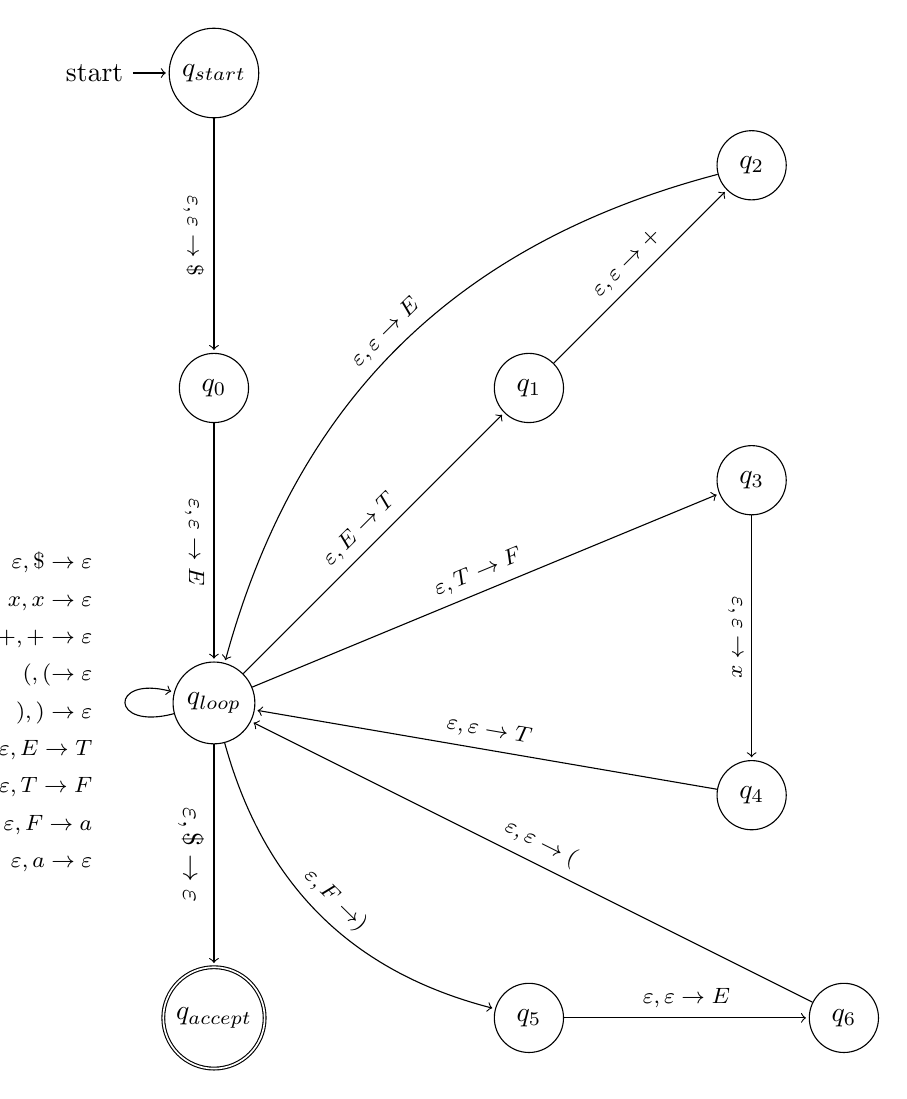
\begin{tikzpicture}[shorten >=1pt,node distance=4cm,on grid,auto]
      \node[state,initial] (q_start) {$q_{start}$};
      \node[state] (q_0) [below=of q_start] {$q_0$};
      \node[state] (q_loop) [below=of q_0] {$q_{loop}$};
      \node[state,accepting] (q_accept) [below=of q_loop] {$q_{accept}$};

      \node[state] (q_1) [right=of q_0] {$q_1$};
      \node[state] (q_2) [above right=of q_1] {$q_2$};

      \node[state] (q_3) [below=of q_2] {$q_3$};
      \node[state] (q_4) [below=of q_3] {$q_4$};

      \node[state] (q_5) [right=of q_accept] {$q_5$};
      \node[state] (q_6) [right=of q_5] {$q_6$};
        \path[->]
          (q_start) edge node [sloped,below] {\footnotesize $\varepsilon,\varepsilon \to \$$} (q_0)
          (q_0) edge node [sloped,below] {\footnotesize $\varepsilon,\varepsilon \to E$} (q_loop)

          (q_loop) edge node [sloped] {\footnotesize $\varepsilon,E \to T$} (q_1)
          (q_1) edge node [sloped] {\footnotesize $\varepsilon,\varepsilon \to +$} (q_2)
          (q_2) edge [bend right] node [sloped] {\footnotesize $\varepsilon,\varepsilon \to E$} (q_loop)

          (q_loop) edge node [sloped] {\footnotesize $\varepsilon,T \to F$} (q_3)
          (q_3) edge node [sloped, below] {\footnotesize $\varepsilon,\varepsilon \to x$} (q_4)
          (q_4) edge node [sloped] {\footnotesize $\varepsilon,\varepsilon \to T$} (q_loop)

          (q_loop) edge [bend right] node [sloped] {\footnotesize $\varepsilon,F \to )$} (q_5)
          (q_5) edge node [sloped] {\footnotesize $\varepsilon,\varepsilon \to E$} (q_6)
          (q_6) edge node [sloped] {\footnotesize $\varepsilon,\varepsilon \to ($} (q_loop)
          
          (q_loop) edge [loop left] node [text width=1cm]
            {\footnotesize
              \begin{itemize}
                \item[$\varepsilon,\$ \to \varepsilon$]
                \item[$x,x \to \varepsilon$]
                \item[$+,+ \to \varepsilon$]
                \item[$(,( \to \varepsilon$]
                \item[$),) \to \varepsilon$]
                \item[$\varepsilon,E \to T$]
                \item[$\varepsilon,T \to F$]
                \item[$\varepsilon,F \to a$]
                \item[$\varepsilon,a \to \varepsilon$]
              \end{itemize}
            } ()
          (q_loop) edge node [sloped, below] {$\varepsilon,\$ \to \varepsilon$} (q_accept);
    \end{tikzpicture}
  \item \textbf{2.13.a -} The grammar will produce a string that alternates between some number of o's, followed by a $\#$ symbol, followed by some number of 0's. That pattern can repeat an infinite number of times. However it can also produce completely different string in which the string starts with n 0's, followed by a $\#$ symbol, followed by 2n 0's.
  \item \textbf{2.14 -} \\
    \textbf{Step 0:} Initial grammar \\
    $A \to BAB | B | \varepsilon$ \\
    $B \to 00 | \varepsilon$ \\
    \\
    \textbf{Step 1:} Insert new start variable \\
    $A_{0} \to A$ \\
    $A \to BAB \mid B \mid \varepsilon$ \\
    $B \to 00 \mid \varepsilon$ \\
    \\
    \textbf{Step 2:} Remove e-rule $B -> \varepsilon$ \\
    $A_{0} \to A$ \\
    $A \to BAB \mid BA \mid AB \mid BB \mid B \mid A \mid \varepsilon$ \\
    $B \to 00$ \\
    \\
    \textbf{Step 3:} Remove e-rule $A \to \varepsilon$ \\
    $A_{0} \to A \mid \varepsilon$ \\
    $A \to BAB \mid BA \mid AB \mid BB \mid B \mid A$ \\
    $B \to 00$ \\
    \\
    \textbf{Step 4:} Remove unit rule $A \to A$ \\
    $A_{0} \to A \mid \varepsilon$ \\
    $A \to BAB \mid BA \mid AB \mid BB \mid B$ \\
    $B \to 00$ \\
    \\
    \textbf{Step 5:} Remove unit rule $A_{0} \to A$ \\
    $A_{0} \to BAB \mid BA \mid AB \mid BB \mid B \mid \varepsilon$ \\
    $A \to BAB \mid BA \mid AB \mid BB \mid B$ \\
    $B \to 00$ \\
    \\
    \textbf{Step 6:} Replace units with terminal\\
    $A_{0} \to BAB \mid BA \mid AB \mid BB \mid 00 \mid \varepsilon$ \\
    $A \to BAB \mid BA \mid AB \mid BB \mid 00$ \\
    $B \to 00$ \\
    \\
    \textbf{Step 7:} Add new terminal \\
    $A_{0} \to BAB \mid BA \mid AB \mid BB \mid CC \mid \varepsilon$ \\
    $A \to BAB \mid BA \mid AB \mid BB \mid CC$ \\
    $B \to CC$ \\
    $C \to 0$ \\
\end{itemize}

\end{document}
